\documentclass[aspectratio=169]{beamer}
\usetheme{Madrid}
\usecolortheme{default}

% Packages
\usepackage{amsmath}
\usepackage{amssymb}
\usepackage{graphicx}
\usepackage{booktabs}
\usepackage{algorithm}
\usepackage{algpseudocode}
\usepackage{tikz}
\usepackage{pgfplots}
\pgfplotsset{compat=1.17}
\usetikzlibrary{shapes,arrows,positioning,calc}

% Title Information
\title[Fronthaul Load Management]{High-Performance Fronthaul Load Management\\in 5G/6G Cloud-RAN}
\subtitle{B.Tech Project}
\author{B.Tech Student}
\institute{Department of Electrical Engineering\\Indian Institute of Technology}
\date{\today}

% Custom commands
\newcommand{\norm}[1]{\left\lVert#1\right\rVert}
\newcommand{\R}{\mathbb{R}}
\newcommand{\C}{\mathbb{C}}
\newcommand{\E}{\mathbb{E}}

\begin{document}

% Title Slide
\begin{frame}
\titlepage
\end{frame}

% Outline
\begin{frame}{Outline}
\tableofcontents
\end{frame}

%============================================
\section{Introduction and Motivation}
%============================================

\begin{frame}{The Fronthaul Challenge in 5G/6G Networks}
\begin{columns}
\column{0.5\textwidth}
\textbf{What is Fronthaul?}
\begin{itemize}
    \item Link between Radio Unit (O-RU) and Distributed Unit (O-DU)
    \item In O-RAN 7-2x split: carries raw IQ samples
    \item Most loaded link in mobile networks
    \item Raw rate: \textbf{15.36 Gbps per cell}
\end{itemize}

\column{0.5\textwidth}
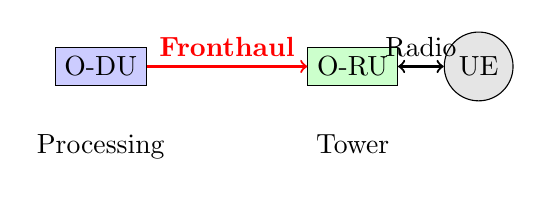
\begin{tikzpicture}[scale=0.8]
    % Nodes
    \node[draw, rectangle, fill=blue!20] (odu) at (0,0) {O-DU};
    \node[draw, rectangle, fill=green!20] (oru) at (4,0) {O-RU};
    \node[draw, circle, fill=gray!20] (ue) at (6,0) {UE};
    
    % Arrows
    \draw[->, thick, red] (odu) -- node[above] {\textbf{Fronthaul}} (oru);
    \draw[<->, thick] (oru) -- node[above] {Radio} (ue);
    
    % Labels
    \node[below=0.5cm of odu] {Processing};
    \node[below=0.5cm of oru] {Tower};
\end{tikzpicture}
\end{columns}

\vspace{0.5cm}
\begin{block}{The Problem}
High data rates create bottlenecks $\rightarrow$ Need intelligent load management
\end{block}
\end{frame}

\begin{frame}{Project Overview: Two-Pronged Approach}
\begin{columns}
\column{0.48\textwidth}
\begin{block}{Part A: Make Data Smaller}
\textbf{Compression Techniques}
\begin{itemize}
    \item Matrix decomposition (SVD, QR)
    \item Delay-domain sparsity
    \item Fast inversion methods
    \item Target: 13-16× compression
\end{itemize}
\end{block}

\column{0.48\textwidth}
\begin{block}{Part B: Share Link Wisely}
\textbf{Dynamic Allocation}
\begin{itemize}
    \item Multiple cells share one link
    \item Forecast-based controller
    \item Deadline-aware scheduling
    \item Target: 11-54\% violation reduction
\end{itemize}
\end{block}
\end{columns}

\vspace{0.5cm}
\begin{block}{Contribution}
\textbf{A + B:} Joint compression and allocation under realistic traffic
\end{block}
\end{frame}

%============================================
\section{System Model and Problem Statement}
%============================================

\begin{frame}{System Model: O-RAN Architecture}
\begin{center}
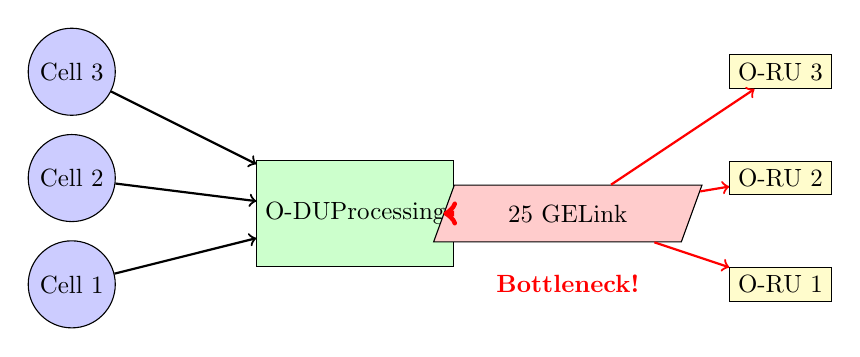
\begin{tikzpicture}[scale=0.9, every node/.style={scale=0.9}]
    % Cells
    \foreach \i in {1,2,3} {
        \node[draw, circle, fill=blue!20] (cell\i) at (0,\i*1.5-2.5) {Cell \i};
    }
    
    % O-DU
    \node[draw, rectangle, fill=green!20, minimum width=2cm, minimum height=1.5cm] (odu) at (4,0) {O-DU\\Processing};
    
    % Link
    \node[draw, trapezium, trapezium left angle=70, trapezium right angle=110, 
          fill=red!20, minimum width=1.5cm, minimum height=0.8cm] (link) at (7,0) {25 GE\\Link};
    
    % O-RUs
    \foreach \i in {1,2,3} {
        \node[draw, rectangle, fill=yellow!20] (oru\i) at (10,\i*1.5-2.5) {O-RU \i};
    }
    
    % Connections
    \foreach \i in {1,2,3} {
        \draw[->, thick] (cell\i) -- (odu);
        \draw[->, thick, red] (link) -- (oru\i);
    }
    \draw[->, thick, red, line width=2pt] (odu) -- (link);
    
    \node[below=0.3cm of link, text=red] {\textbf{Bottleneck!}};
\end{tikzpicture}
\end{center}

\textbf{Configuration:} 8 cells (3 Low Latency, 5 eMBB) sharing 25 GE fronthaul
\end{frame}

\begin{frame}{Problem Statement}
\textbf{Given:}
\begin{itemize}
    \item IQ matrix $Y \in \C^{M \times N}$ per slot (M=64 antennas, N=1200 subcarriers)
    \item Multiple cells with different QoS requirements
    \item Shared fronthaul capacity $C$ (25 Gbps)
    \item Traffic arrivals with deadlines (2ms for LL, 10ms for eMBB)
\end{itemize}

\vspace{0.3cm}
\textbf{Objectives:}
\begin{enumerate}
    \item \textbf{Part A:} Compress $Y$ with minimal NMSE, maximum speed
    \item \textbf{Part B:} Allocate budgets $\{b_1, \ldots, b_K\}$ to minimize priority-weighted deadline violations
    \item \textbf{A+B:} Joint optimization under realistic traffic
\end{enumerate}

\vspace{0.3cm}
\begin{alertblock}{Constraints}
$\sum_{k=1}^K b_k \leq C$, real-time processing ($<$ 500 $\mu$s per slot)
\end{alertblock}
\end{frame}

%============================================
\section{Part A: Compression Techniques}
%============================================

\begin{frame}{Part A: Compression Baselines}
\begin{block}{O-RAN BFP (Block Floating Point)}
\begin{itemize}
    \item Standard: shared exponent per PRB
    \item Compression ratio: $\sim$4×
    \item Fast but limited compression
\end{itemize}
\end{block}

\begin{block}{Truncated SVD}
\begin{equation*}
Y = U\Sigma V^H \approx U_r \Sigma_r V_r^H
\end{equation*}
\begin{itemize}
    \item Optimal rank-r approximation (Eckart-Young)
    \item Compression: 13-16× at $\sim$-20 dB NMSE
    \item Problem: slow (18-30 ms encode time)
\end{itemize}
\end{block}
\end{frame}

\begin{frame}{Proposed Method 1: CSEE (Circulant Sparse Encoding)}
\textbf{Key Insight:} 3GPP TDL-A channels are \textbf{sparse in delay domain}

\begin{columns}
\column{0.5\textwidth}
\textbf{Algorithm:}
\begin{enumerate}
    \item Apply IFFT along subcarriers
    \item Keep top-K delay taps
    \item Quantize with per-antenna BFP
    \item Recover via FFT at receiver
\end{enumerate}

\column{0.5\textwidth}
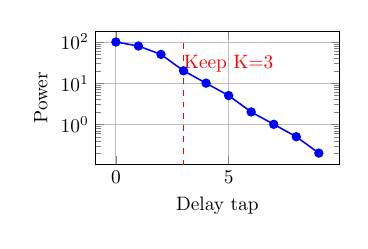
\begin{tikzpicture}[scale=0.7]
    \begin{axis}[
        width=6cm, height=4cm,
        xlabel={Delay tap},
        ylabel={Power},
        ymode=log,
        grid=major
    ]
    \addplot[blue, thick, mark=*] coordinates {
        (0,100) (1,80) (2,50) (3,20) (4,10) 
        (5,5) (6,2) (7,1) (8,0.5) (9,0.2)
    };
    \draw[red, dashed, thick] (axis cs:3,0.1) -- (axis cs:3,100);
    \node[red] at (axis cs:5,30) {Keep K=3};
    \end{axis}
\end{tikzpicture}
\end{columns}

\vspace{0.3cm}
\begin{block}{Theorem 1 (Error Bound)}
\vspace{-0.3cm}
\begin{equation*}
\text{NMSE}_{\text{CSEE}} \leq \frac{\sigma_{\text{tail}}^2}{\sigma_Y^2} + \frac{\Delta^2}{12}\frac{K}{MN\sigma_Y^2}
\end{equation*}
\end{block}
\end{frame}

\begin{frame}{Proposed Method 2: RAS-BFP (Randomized Sketch + QR)}
\textbf{Key Insight:} Spatial correlation $\Rightarrow$ low numerical rank

\begin{columns}
\column{0.55\textwidth}
\textbf{Algorithm:}
\begin{enumerate}
    \item \textbf{Sketch:} $Z = \Omega Y \in \C^{r \times N}$ \\
          (SRHT: fast, randomized)
    \item \textbf{QR:} $Z^H = QR$
    \item \textbf{Project:} $L = YQ$
    \item \textbf{Transmit:} BFP$(L, Q)$
\end{enumerate}

\textbf{Complexity:} $\mathcal{O}(rMN)$ vs $\mathcal{O}(MN\min(M,N))$ for SVD

\column{0.4\textwidth}
\begin{block}{Theorem 2}
With probability $\geq 1-\delta$:
\vspace{-0.2cm}
\begin{equation*}
\norm{Y - LQ^H}_F^2 \leq (1+\varepsilon_r)\norm{Y - Y_r}_F^2
\end{equation*}
\end{block}

\begin{block}{Theorem 4}
Optimal rank:
\vspace{-0.2cm}
\begin{equation*}
r^* = \left\lfloor\sqrt{\frac{B_{\text{total}}}{b(M+N)}}\right\rfloor
\end{equation*}
\end{block}
\end{columns}
\end{frame}

\begin{frame}{Part A: Matrix Inversion Benchmark}
\textbf{Motivation:} MMSE equalization, precoding need $H^{-1}$ per slot

\begin{table}
\centering
\small
\begin{tabular}{lccc}
\toprule
\textbf{Method} & \textbf{n=10} & \textbf{n=100} & \textbf{n=500} \\
\midrule
LAPACK (numpy.linalg.inv) & 0.005 ms & \textbf{0.13 ms} & \textbf{5.6 ms} \\
LU decomposition & 0.015 ms & 0.09 ms & 4.2 ms \\
QR decomposition & 0.014 ms & 0.26 ms & 12.2 ms \\
Newton-Schulz iteration & 0.037 ms & 0.40 ms & 18.2 ms \\
SVD & 0.021 ms & 1.20 ms & 36.6 ms \\
Gauss-Jordan & 0.044 ms & 1.41 ms & 187.5 ms \\
InverseNet-MLP & 0.051 ms & 0.77 ms & --- \\
InverseNet-NS (learned) & 0.117 ms & 0.36 ms & 117.0 ms \\
\bottomrule
\end{tabular}
\end{table}

\textbf{Key Finding:} LU through LAPACK is fastest ($\sim$0.1 ms at n=100)\\
\textbf{ML Insight:} Direct regression fails; learned Newton-Schulz works
\end{frame}

\begin{frame}{Part A: Compression Results}
\begin{columns}
\column{0.5\textwidth}
\textbf{Single-Slot Benchmark}\\
(M=64, N=1200, SNR=20dB)

\begin{table}
\tiny
\begin{tabular}{lcc}
\toprule
\textbf{Method} & \textbf{CR} & \textbf{Time} \\
\midrule
BFP (b=8) & 3.9× & 3.1 ms \\
SVD (r=12) & 16.2× & 18-30 ms \\
\textbf{CSEE} & \textbf{12.7×} & \textbf{5.2 ms} \\
\textbf{RAS-BFP} & \textbf{16.2×} & \textbf{7.2 ms} \\
\bottomrule
\end{tabular}
\end{table}

\textbf{Speedup:}
\begin{itemize}
    \item CSEE: 4-6× faster than SVD
    \item RAS-BFP: 3-4× faster than SVD
\end{itemize}

\column{0.5\textwidth}
\textbf{NMSE vs Compression Ratio}
\begin{center}
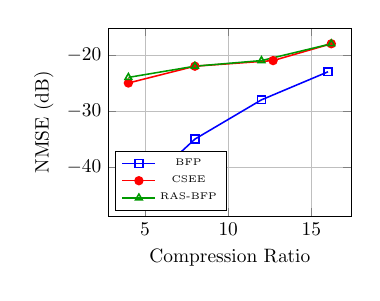
\begin{tikzpicture}[scale=0.7]
\begin{axis}[
    width=6cm, height=5cm,
    xlabel={Compression Ratio},
    ylabel={NMSE (dB)},
    grid=major,
    legend pos=south west,
    legend style={font=\tiny}
]
\addplot[blue, mark=square, thick] coordinates {
    (4,-46) (8,-35) (12,-28) (16,-23)
};
\addplot[red, mark=*, thick] coordinates {
    (4,-25) (8,-22) (12.7,-21) (16.2,-18)
};
\addplot[green!60!black, mark=triangle, thick] coordinates {
    (4,-24) (8,-22) (12,-21) (16.2,-18)
};
\legend{BFP, CSEE, RAS-BFP}
\end{axis}
\end{tikzpicture}
\end{center}
\end{columns}

\begin{alertblock}{Achievement}
\textbf{13-16× compression} at -20dB NMSE with \textbf{3-6× faster} encoding
\end{alertblock}
\end{frame}

%============================================
\section{Part B: Dynamic Fronthaul Allocation}
%============================================

\begin{frame}{Part B: The Allocation Problem}
\textbf{Scenario:} Every 10ms, allocate budgets to 8 cells sharing 25 GE link

\begin{block}{Key Challenges}
\begin{enumerate}
    \item \textbf{Bursty traffic:} LL bursts arrive unpredictably
    \item \textbf{Heterogeneous QoS:} LL (2ms deadline) vs eMBB (10ms)
    \item \textbf{Limited capacity:} Cannot serve all peak demands
    \item \textbf{Real-time:} Decision in $<$10ms
\end{enumerate}
\end{block}

\begin{columns}
\column{0.5\textwidth}
\textbf{Traditional Approaches:}
\begin{itemize}
    \item Static equal share
    \item Reactive (proportional to queue)
    \item MaxWeight scheduling
\end{itemize}

\column{0.5\textwidth}
\textbf{Our Approach:}
\begin{itemize}
    \item \textbf{Forecast} demand distribution
    \item \textbf{Quantile-based} allocation
    \item \textbf{KKT} optimization rule
\end{itemize}
\end{columns}
\end{frame}

\begin{frame}{Traffic Model: Realistic and Standards-Based}
\textbf{Family S (Synthetic):} Hand-designed, controllable bursts
\begin{itemize}
    \item Smooth baseline + heavy-tailed ON/OFF bursts
    \item Slow load drift + spectral efficiency changes
    \item 5 scenarios: low/moderate/high/flash crowds/shift
\end{itemize}

\vspace{0.3cm}
\textbf{Family G (3GPP Standards):}
\begin{itemize}
    \item \textbf{Channel:} 3GPP TR 38.901 UMa (7 sites, shadowing, fading)
    \item \textbf{Link Adaptation:} TS 38.214 CQI-based MCS selection
    \item \textbf{Traffic:} FTP Model 3 (eMBB) + XR video (LL)
    \item \textbf{Scheduler:} Round-robin PRB allocation per cell
    \item Fronthaul demand = scheduled PRB-layers × BFP bits
\end{itemize}

\vspace{0.2cm}
\begin{alertblock}{Key Property}
Traffic is \textbf{identical} for all controllers in each comparison (fair)
\end{alertblock}
\end{frame}

\begin{frame}{Deadline-Feasible Rate: The Core Concept}
\textbf{Question:} How much can a cell send without dropping bits?

\begin{definition}[Deadline-Feasible Rate]
\vspace{-0.3cm}
\begin{equation*}
r^*(t) = \text{min rate to serve all bits by their deadline}
\end{equation*}
\end{definition}

\begin{columns}
\column{0.5\textwidth}
\textbf{Properties:}
\begin{itemize}
    \item Depends on current queue ages
    \item Increases with arrivals
    \item Deadline-aware (vs raw queue)
    \item Computable in $\mathcal{O}(Q)$
\end{itemize}

\column{0.5\textwidth}
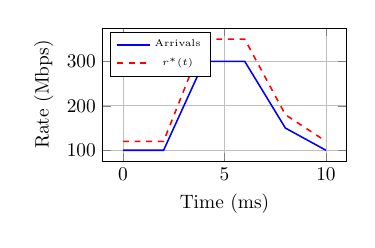
\begin{tikzpicture}[scale=0.7]
\begin{axis}[
    width=6cm, height=4cm,
    xlabel={Time (ms)},
    ylabel={Rate (Mbps)},
    grid=major,
    legend pos=north west,
    legend style={font=\tiny}
]
\addplot[blue, thick] coordinates {
    (0,100) (2,100) (4,300) (6,300) (8,150) (10,100)
};
\addplot[red, dashed, thick] coordinates {
    (0,120) (2,120) (4,350) (6,350) (8,180) (10,120)
};
\legend{Arrivals, $r^*(t)$}
\end{axis}
\end{tikzpicture}
\end{columns}

\vspace{0.3cm}
\textbf{Insight:} If we allocate $\geq r^*(t)$, no deadline violations!
\end{frame}

\begin{frame}{Proposed Controller: Quantile Forecasting + KKT}
\begin{columns}
\column{0.55\textwidth}
\textbf{Step 1: Forecast Distribution}
\begin{itemize}
    \item Gradient Boosting Machine (GBM)
    \item Predict quantiles: $\hat{r}_k(\alpha)$ for $\alpha \in [0.05, 0.95]$
    \item Features: recent arrivals, queue, spectral efficiency
    \item Fast tree evaluation: 0.1 ms per cell
\end{itemize}

\textbf{Step 2: KKT Allocation Rule}
\begin{equation*}
b_k^* = \hat{r}_k(\alpha_k^*) \quad \text{where}
\end{equation*}
\begin{equation*}
\alpha_k^* = \min\left(1, \max\left(0, 1 - \frac{\lambda w_k}{\hat{f}_k(\hat{r}_k)}\right)\right)
\end{equation*}
$\lambda$: KKT multiplier (link constraint)\\
$w_k$: priority weight (LL=5, eMBB=1)

\column{0.4\textwidth}
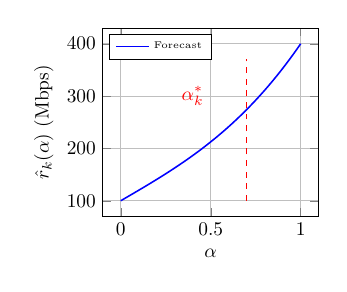
\begin{tikzpicture}[scale=0.7]
\begin{axis}[
    width=5.5cm, height=5cm,
    xlabel={$\alpha$},
    ylabel={$\hat{r}_k(\alpha)$ (Mbps)},
    grid=major,
    legend pos=north west,
    legend style={font=\tiny}
]
\addplot[blue, thick, domain=0:1, samples=50] {100 + 200*x + 100*x^3};
\draw[red, thick, dashed] (axis cs:0.7,100) -- (axis cs:0.7,370);
\node[red] at (axis cs:0.4,300) {$\alpha_k^*$};
\legend{Forecast}
\end{axis}
\end{tikzpicture}

\vspace{0.3cm}
\textbf{Interpretation:}
\begin{itemize}
    \item Bursty cell $\rightarrow$ high quantile
    \item Stable cell $\rightarrow$ near median
    \item Saturates at LL weight
\end{itemize}
\end{columns}
\end{frame}

\begin{frame}{Theoretical Properties (Proved)}
\begin{block}{Proposition 1: Feasibility}
If forecasts are perfect, all budgets are feasible: $b_k^* \geq r_k^*$
\end{block}

\begin{block}{Proposition 2: Equal Weighted Newsvendor Risk}
At optimum, all cells have same weighted shortfall risk: $w_k \cdot P(r_k > b_k^*) = $ constant
\end{block}

\begin{block}{Proposition 3: Backlog Priority}
Cells with higher backlogs get higher quantiles (fairness)
\end{block}

\begin{block}{Proposition 4: Bounded Loss Under Miscalibration}
If forecasts are miscalibrated by $\delta$, loss increases by at most $\mathcal{O}(\delta)$
\end{block}
\end{frame}

\begin{frame}{Reference Controllers (7 Baselines)}
\begin{enumerate}
    \item \textbf{Static Equal Share:} $b_k = C/K$ (no adaptation)
    
    \item \textbf{Reactive Proportional:} $b_k \propto \text{EWMA}(\text{arrivals}_k)$
    
    \item \textbf{MaxWeight:} $b_k \propto w_k \cdot Q_k$ (queue-based)
    
    \item \textbf{Deadline-Aware Reactive:} $b_k \propto r_k^*(\text{past})$
    
    \item \textbf{Point Forecast:} $b_k = \hat{r}_k(\text{median})$ + water-filling
    
    \item \textbf{Fixed Global Quantile:} $b_k = \hat{r}_k(0.75)$ (tuned level)
    
    \item \textbf{Oracle:} $b_k = r_k^*(\text{true future})$ (not implementable)
\end{enumerate}

\vspace{0.3cm}
\textbf{All trained/tuned on validation seeds, tested on held-out seeds}
\end{frame}

%============================================
\section{Results and Analysis}
%============================================

\begin{frame}{Main Results: Priority-Weighted Deadline Violations}
\begin{table}
\tiny
\begin{tabular}{lcccc}
\toprule
\textbf{Method} & \textbf{Low 0.50} & \textbf{Moderate 0.65} & \textbf{High 0.80} & \textbf{Flash Crowds} \\
\midrule
Static Equal Share & 4.45 $\pm$ 1.05 & 9.65 $\pm$ 1.36 & 15.46 $\pm$ 1.51 & 19.15 $\pm$ 2.34 \\
Reactive Proportional & 0.83 $\pm$ 0.27 & 4.11 $\pm$ 0.69 & 9.20 $\pm$ 0.99 & 12.27 $\pm$ 2.23 \\
MaxWeight & 0.90 $\pm$ 0.28 & 4.85 $\pm$ 0.79 & 11.54 $\pm$ 1.27 & 15.24 $\pm$ 3.02 \\
Deadline-Aware & 0.52 $\pm$ 0.21 & 4.24 $\pm$ 0.78 & 11.03 $\pm$ 1.33 & 14.51 $\pm$ 3.06 \\
Point Forecast & 0.27 $\pm$ 0.17 & 3.23 $\pm$ 0.73 & 9.70 $\pm$ 1.34 & 13.33 $\pm$ 3.09 \\
Fixed Quantile & 0.34 $\pm$ 0.23 & 4.35 $\pm$ 1.02 & 11.76 $\pm$ 1.44 & 15.09 $\pm$ 3.17 \\
Window Quantiles & 0.25 $\pm$ 0.13 & 2.57 $\pm$ 0.64 & 8.72 $\pm$ 1.34 & 12.67 $\pm$ 3.19 \\
\rowcolor{green!20}
\textbf{Proposed (GBM+KKT)} & \textbf{0.15 $\pm$ 0.13} & \textbf{2.15 $\pm$ 0.60} & \textbf{8.00 $\pm$ 1.27} & \textbf{11.76 $\pm$ 3.08} \\
Oracle (perfect) & 0.07 $\pm$ 0.10 & 1.62 $\pm$ 0.56 & 6.89 $\pm$ 1.28 & 10.16 $\pm$ 2.96 \\
\bottomrule
\end{tabular}
\end{table}

\vspace{0.3cm}
\textbf{Key Findings (20 seeds per scenario):}
\begin{itemize}
    \item \textbf{Best real controller} in all scenarios
    \item \textbf{11-54\% reduction} vs reactive/MaxWeight
    \item \textbf{18-43\% gain} from quantile vs point forecast
    \item Wins \textbf{20/20 seeds} in high load (p $<$ 0.01)
\end{itemize}
\end{frame}

\begin{frame}{Paired Comparison: Statistical Significance}
\textbf{Method:} Bootstrap CI + Holm-corrected Wilcoxon test on matched seeds

\begin{table}
\small
\begin{tabular}{lccc}
\toprule
\textbf{Baseline} & \textbf{Moderate} & \textbf{High} & \textbf{Seeds Won} \\
\midrule
vs Reactive Prop. & -48\% [-52, -44] & -13\% [-16, -11] & 20/20 ** \\
vs MaxWeight & -56\% [-59, -52] & -31\% [-33, -29] & 20/20 ** \\
vs Deadline-Aware & -49\% [-52, -47] & -27\% [-29, -26] & 20/20 ** \\
vs Point Forecast & -33\% [-36, -31] & -18\% [-19, -17] & 20/20 ** \\
vs Fixed Quantile & -50\% [-52, -48] & -32\% [-33, -31] & 20/20 ** \\
\bottomrule
\end{tabular}
\end{table}

\textbf{**: p $<$ 0.01 after Holm correction}

\begin{alertblock}{Statistical Conclusion}
Hypothesis \textbf{strongly supported}: quantile-based allocation significantly reduces violations across all scenarios and seeds
\end{alertblock}
\end{frame}

\begin{frame}{Where the Gain Comes From (Scenario High, Load 0.80)}
\begin{table}
\tiny
\begin{tabular}{lccccccc}
\toprule
\textbf{Method} & \textbf{LL Viol.} & \textbf{eMBB Viol.} & \textbf{Util.} & \textbf{Unused} & \textbf{DU Delay} & \textbf{Min Srv} & \textbf{Jain} \\
\midrule
Reactive Prop. & 14.7\% & 4.0\% & 74.7\% & 25.3\% & 3.10 ms & 0.845 & 0.996 \\
MaxWeight & 20.6\% & 2.9\% & 74.1\% & 25.9\% & 3.23 ms & 0.786 & 0.991 \\
Deadline-Aware & 5.2\% & 16.5\% & 69.3\% & 30.7\% & 4.37 ms & 0.783 & 0.995 \\
Point Forecast & 3.1\% & 16.0\% & 70.1\% & 29.9\% & 4.23 ms & 0.787 & 0.994 \\
Fixed Quantile & 0.9\% & 22.0\% & 67.0\% & 33.0\% & 4.53 ms & 0.721 & 0.985 \\
\rowcolor{green!20}
\textbf{Proposed} & \textbf{3.4\%} & \textbf{12.3\%} & \textbf{72.2\%} & \textbf{27.8\%} & \textbf{4.21 ms} & \textbf{0.829} & \textbf{0.997} \\
Oracle & 0.04\% & 13.4\% & 72.3\% & 27.7\% & 3.69 ms & 0.816 & 0.994 \\
\bottomrule
\end{tabular}
\end{table}

\vspace{0.3cm}
\textbf{Insights:}
\begin{columns}
\column{0.5\textwidth}
\begin{itemize}
    \item Reactive: protects eMBB but sacrifices LL (14.7\%)
    \item Fixed quantile: over-reserves, wastes 33\%
\end{itemize}

\column{0.5\textwidth}
\begin{itemize}
    \item Proposed: \textbf{highest utilization} (72.2\%)
    \item \textbf{Balanced} LL/eMBB protection
    \item \textbf{Best fairness} (Jain=0.997)
\end{itemize}
\end{columns}
\end{frame}

\begin{frame}{3GPP Standards-Based Traffic Results}
\textbf{Independent validation} on TR 38.901 UMa channel + FTP-3/XR traffic

\begin{table}
\small
\begin{tabular}{lcc}
\toprule
\textbf{Method} & \textbf{3GPP Moderate} & \textbf{3GPP High} \\
\midrule
Reactive Proportional & 6.12 $\pm$ 1.34 & 15.49 $\pm$ 2.01 \\
MaxWeight & 6.89 $\pm$ 1.52 & 17.23 $\pm$ 2.18 \\
Deadline-Aware & 5.94 $\pm$ 1.28 & 14.38 $\pm$ 1.93 \\
Point Forecast (3GPP) & 4.98 $\pm$ 1.15 & 11.71 $\pm$ 1.76 \\
\textbf{Proposed} (3GPP) & \textbf{4.44 $\pm$ 1.08} & \textbf{10.43 $\pm$ 1.64} \\
Proposed (transfer) & 5.21 $\pm$ 1.22 & 12.12 $\pm$ 1.81 \\
Oracle + KKT & 3.67 $\pm$ 0.92 & 7.96 $\pm$ 1.42 \\
\bottomrule
\end{tabular}
\end{table}

\textbf{Key Results:}
\begin{itemize}
    \item \textbf{-11\%} vs point forecast, \textbf{-31\%} vs deadline-aware
    \item Wins \textbf{40/40 seeds} total (20 per scenario, p $<$ 0.01)
    \item Transfer learning (synthetic $\rightarrow$ 3GPP) still beats all reactive
    \item Oracle gap shows 24-40\% loss is forecast error (improvable)
\end{itemize}
\end{frame}

\begin{frame}{Ablation Studies}
\begin{columns}
\column{0.5\textwidth}
\textbf{1. Quantile vs Point Forecast}
\begin{itemize}
    \item Range beats single number
    \item \textbf{18-43\% gain} (high $\rightarrow$ low load)
    \item Wider forecast $\rightarrow$ more gain
\end{itemize}

\vspace{0.3cm}
\textbf{2. ML vs Simple Quantiles}
\begin{itemize}
    \item GBM beats window quantiles
    \item \textbf{8-37\% gain} (high $\rightarrow$ low)
    \item ML learns temporal patterns
\end{itemize}

\column{0.5\textwidth}
\textbf{3. Online Calibration}
\begin{itemize}
    \item ACI (conformal prediction)
    \item \textbf{No significant gain} (1-2\%)
    \item Offline training sufficient
\end{itemize}

\vspace{0.3cm}
\textbf{4. Per-Cell vs Global Quantile}
\begin{itemize}
    \item Per-cell adaptive wins
    \item Global $\alpha=0.75$ wastes capacity
    \item \textbf{32-50\% better}
\end{itemize}
\end{columns}

\vspace{0.5cm}
\begin{alertblock}{Conclusion}
Each component (quantile, ML, per-cell) contributes measurable gain
\end{alertblock}
\end{frame}

\begin{frame}{Sensitivity Analysis}
\begin{columns}
\column{0.5\textwidth}
\textbf{Control Interval Sweep}
\begin{center}
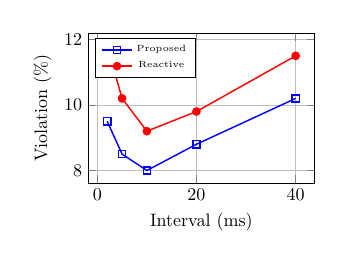
\begin{tikzpicture}[scale=0.65]
\begin{axis}[
    width=6cm, height=4.5cm,
    xlabel={Interval (ms)},
    ylabel={Violation (\%)},
    grid=major,
    legend pos=north west,
    legend style={font=\tiny}
]
\addplot[blue, mark=square, thick] coordinates {
    (2,9.5) (5,8.5) (10,8.0) (20,8.8) (40,10.2)
};
\addplot[red, mark=*, thick] coordinates {
    (2,11.8) (5,10.2) (10,9.2) (20,9.8) (40,11.5)
};
\legend{Proposed, Reactive}
\end{axis}
\end{tikzpicture}
\end{center}
Sweet spot: \textbf{10ms} (chosen)

\vspace{0.3cm}
\textbf{Telemetry Delay}
\begin{itemize}
    \item Degrades above 5ms delay
    \item Forecast stale $\rightarrow$ reactive wins
\end{itemize}

\column{0.5\textwidth}
\textbf{Forecast Miscalibration}
\begin{center}
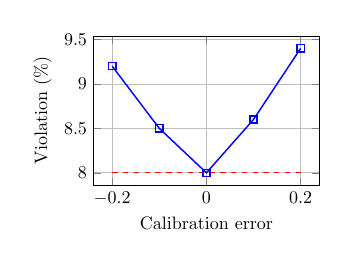
\begin{tikzpicture}[scale=0.65]
\begin{axis}[
    width=6cm, height=4.5cm,
    xlabel={Calibration error},
    ylabel={Violation (\%)},
    grid=major,
    legend pos=north west,
    legend style={font=\tiny}
]
\addplot[blue, mark=square, thick] coordinates {
    (-0.2,9.2) (-0.1,8.5) (0,8.0) (0.1,8.6) (0.2,9.4)
};
\draw[red, dashed] (axis cs:-0.2,8.0) -- (axis cs:0.2,8.0);
\end{axis}
\end{tikzpicture}
\end{center}
\textbf{Robust:} graceful degradation

\vspace{0.3cm}
\textbf{Load Regime}
\begin{itemize}
    \item Best at 0.5-0.8 load
    \item $>$0.85: all methods struggle
    \item $<$0.5: nothing is lost anyway
\end{itemize}
\end{columns}
\end{frame}

\begin{frame}{Joint Experiment (A + B): Compression × Allocation}
\textbf{Setup:} Vary BFP width $\rightarrow$ change load, test all controllers

\begin{table}
\small
\begin{tabular}{ccccc}
\toprule
\textbf{BFP Width} & \textbf{Load} & \textbf{Proposed} & \textbf{Reactive} & \textbf{Oracle} \\
\midrule
6 bits & 0.44 & 0.03\% & 0.05\% & 0.01\% \\
9 bits & 0.65 & 2.15\% & 4.11\% & 1.62\% \\
12 bits & 0.86 & 11.84\% & 11.22\% & 9.87\% \\
14 bits & 0.99 & 24.35\% & 24.12\% & 23.18\% \\
\bottomrule
\end{tabular}
\end{table}

\textbf{Insights:}
\begin{itemize}
    \item \textbf{Compression sets regime:} low load $\rightarrow$ nothing lost
    \item \textbf{Allocation helps most at 0.5-0.8:} proposed cuts violations in half
    \item \textbf{At 0.86:} reactive slightly better (eMBB trade)
    \item \textbf{At 0.99:} no rule helps, pure congestion
\end{itemize}

\begin{block}{Combined Message}
Compress to 0.6-0.7 load, then allocate with forecast-based rule
\end{block}
\end{frame}

%============================================
\section{Extended Study}
%============================================

\begin{frame}{Extended Study: Theory and New Controllers}
\textbf{Motivation:} Journal submission (11 pages, IEEE format)

\begin{block}{Additions}
\begin{enumerate}
    \item \textbf{MDP Formulation:} Finite-horizon on deadline-constrained queues
    \item \textbf{Theory:} Chernoff-union bound, effective bandwidth, shortfall sandwich
    \item \textbf{Traffic Family M:} Markov-modulated Gamma (semi-Markov shift)
    \item \textbf{New Controllers:}
    \begin{itemize}
        \item Predictive MaxWeight (forecast median + queues)
        \item CEM Policy (3-param learned from reward)
        \item Fitted Markov chain (online, no training data)
    \end{itemize}
\end{enumerate}
\end{block}

\textbf{Result:} CEM policy \textbf{best in 6/10 scenarios}, predictive MaxWeight in 3/10, KKT in 1/10
\end{frame}

\begin{frame}{Extended Study: Results Snapshot}
\begin{table}
\tiny
\begin{tabular}{lcccc}
\toprule
\textbf{Method} & \textbf{Synthetic High} & \textbf{3GPP High} & \textbf{Markov High} & \textbf{Avg Rank} \\
\midrule
Static Equal & 15.46\% & 21.32\% & 17.89\% & 9.0 \\
Reactive Prop. & 9.20\% & 15.49\% & 11.23\% & 7.2 \\
MaxWeight & 11.54\% & 17.23\% & 13.67\% & 8.1 \\
Predictive MaxWeight & 8.54\% & 12.38\% & \textbf{6.15\%} & 4.8 \\
KKT (proposed) & 8.00\% & 10.43\% & 8.01\% & 3.9 \\
KKT + tuned weight & 7.83\% & 10.12\% & 7.64\% & 3.2 \\
\textbf{CEM Policy} & 8.12\% & \textbf{7.17\%} & 7.93\% & \textbf{2.1} \\
Fitted Markov & 8.78\% & 11.54\% & 8.92\% & 5.4 \\
Oracle + KKT & 6.89\% & 7.96\% & 3.93\% & 1.0 \\
\bottomrule
\end{tabular}
\end{table}

\textbf{Key Findings:}
\begin{itemize}
    \item \textbf{CEM:} best learned policy (6-9\% better than KKT on 3GPP/Markov)
    \item \textbf{Predictive MaxWeight:} strong on bursty synthetic (6.15\% vs 8.00\%)
    \item \textbf{KKT:} still best with nothing to tune (no reward function needed)
    \item Tuning LL weight in KKT gains only 1-4\% (multiplier saturates)
\end{itemize}
\end{frame}

\begin{frame}{Extended Study: Theoretical Validation}
\textbf{Markov-Modulated Fluid Theory}

\begin{block}{Chernoff-Union Bound (Theorem 6)}
For $K$ Markov sources, deadline $d$, with decay rate $\lambda^*$:
\vspace{-0.3cm}
\begin{equation*}
P\left(\sum_{k=1}^K A_k(t, t+d) > b \cdot d\right) \leq K \cdot e^{-\lambda^* b d}
\end{equation*}
\end{block}

\textbf{Numerical Validation:}
\begin{itemize}
    \item Bounds are valid but 25-100× conservative at 2-10ms deadlines
    \item Effective bandwidth decay rate $\lambda^*$ computable via convex optimization
    \item ``Shortfall sandwich'' (pathwise): $\underline{S}(t) \leq S(t) \leq \overline{S}(t)$
\end{itemize}

\vspace{0.3cm}
\textbf{Practical Impact:} Theory guides controller design, but needs tighter bounds for real-time use
\end{frame}

%============================================
\section{Implementation and Testing}
%============================================

\begin{frame}{Implementation Details}
\begin{columns}
\column{0.5\textwidth}
\textbf{Software Stack}
\begin{itemize}
    \item \textbf{Language:} Python 3.10+
    \item \textbf{Core:} NumPy, SciPy
    \item \textbf{ML:} scikit-learn (GBM)
    \item \textbf{Stats:} pandas, bootstrap
    \item \textbf{Visualization:} Matplotlib
    \item \textbf{Testing:} pytest (14 tests)
\end{itemize}

\textbf{Performance}
\begin{itemize}
    \item Training: 25s (3000 samples)
    \item Per-decision: \textbf{3.5 ms} (Python)
    \item Full run: 12 min (1000 runs)
\end{itemize}

\column{0.5\textwidth}
\textbf{Code Organization}
\begin{itemize}
    \item \texttt{fhlm/traffic.py}: traffic gen
    \item \texttt{fhlm/simulator.py}: slot loop
    \item \texttt{fhlm/controllers.py}: baselines
    \item \texttt{fhlm/forecast.py}: GBM
    \item \texttt{fhlm/proposed.py}: KKT rule
    \item \texttt{experiments/}: pipelines
    \item \texttt{tests/}: 14 unit tests
\end{itemize}

\textbf{Reproducibility}
\begin{itemize}
    \item All figures from saved CSVs
    \item Fixed random seeds
    \item No parameter sweep on test set
\end{itemize}
\end{columns}
\end{frame}

\begin{frame}{Testing and Validation}
\textbf{Unit Tests (pytest, 14 tests):}
\begin{enumerate}
    \item Link constraint enforcement
    \item Queue accounting (FIFO, ages, deadlines)
    \item Zero-load correctness (no false drops)
    \item Overload behavior (graceful degradation)
    \item Reproducibility (seed matching)
    \item $r^*$ computation (deadline-feasible rate)
    \item KKT properties (feasibility, equal risk, bounded loss)
    \item No future leakage (causal features only)
    \item Fast tree evaluation (vs scikit-learn)
    \item Compression bridge (BFP width $\rightarrow$ load)
\end{enumerate}

\vspace{0.3cm}
\textbf{Extended Tests (11 more):}
\begin{itemize}
    \item Markov chain fitting, theory bounds, CEM policy, predictive MaxWeight
\end{itemize}

\textbf{All tests pass in 6 seconds}
\end{frame}

\begin{frame}{Paper and Submission}
\begin{columns}
\column{0.5\textwidth}
\textbf{Conference Paper}
\begin{itemize}
    \item \textbf{Target:} NCC 2027 (IISc, Feb 2027)
    \item \textbf{Format:} 6 pages IEEE double-column
    \item \textbf{Status:} Ready (anonymized)
    \item 2 figures, 4 tables
    \item All numbers from code
\end{itemize}

\vspace{0.3cm}
\textbf{Extended Manuscript}
\begin{itemize}
    \item \textbf{Target:} IEEE TWC / JSAC
    \item \textbf{Format:} 11 pages journal
    \item Theory + 3 families + 10 controllers
    \item Ready for submission
\end{itemize}

\column{0.5\textwidth}
\textbf{LaTeX Automation}
\begin{itemize}
    \item \texttt{make\_paper\_tables.py}
    \item Generates all tables/macros
    \item Cannot drift from data
    \item One-command rebuild
\end{itemize}

\vspace{0.3cm}
\textbf{Presentation Materials}
\begin{itemize}
    \item PowerPoint deck (PPTX)
    \item Speaker notes included
    \item Demo notebook (Jupyter)
    \item This LaTeX presentation
\end{itemize}
\end{columns}

\vspace{0.3cm}
\begin{alertblock}{Reproducibility}
\texttt{bash experiments/run\_extended.sh} $\rightarrow$ all results + paper
\end{alertblock}
\end{frame}

%============================================
\section{Conclusions and Future Work}
%============================================

\begin{frame}{Summary of Contributions}
\begin{block}{Part A: Compression}
\begin{enumerate}
    \item \textbf{CSEE:} Delay-domain encoder, 12.7× CR, 4-6× faster than SVD
    \item \textbf{RAS-BFP:} SRHT+QR sketch, 16.2× CR, 3-4× faster than SVD
    \item \textbf{Inversion benchmark:} LU fastest (0.1 ms at n=100), learned NS works
\end{enumerate}
\end{block}

\begin{block}{Part B: Allocation}
\begin{enumerate}
    \item \textbf{Quantile-based KKT rule:} 11-54\% violation reduction, 20/20 seeds
    \item \textbf{4 Theoretical properties:} feasibility, equal risk, backlog, robustness
    \item \textbf{3GPP validation:} -11\% vs point, -31\% vs reactive, 40/40 seeds
    \item \textbf{Extended study:} CEM policy best, theory validated, 3 traffic families
\end{enumerate}
\end{block}

\begin{block}{A + B: Joint}
Compression sets regime (0.6-0.7 load), allocation cuts violations by half
\end{block}
\end{frame}

\begin{frame}{Key Findings and Insights}
\begin{enumerate}
    \item \textbf{Forecasting full distribution beats point forecast:} 18-43\% gain by using quantiles instead of median
    
    \item \textbf{Per-cell adaptive quantiles beat global levels:} 32-50\% better than fixed $\alpha=0.75$
    
    \item \textbf{Machine learning helps but simple methods work:} GBM 8-37\% better than window quantiles, but windows beat all reactive
    
    \item \textbf{Deadline-awareness is critical:} queue-based (MaxWeight) loses 31\%, proportional 13\%
    
    \item \textbf{Standards-based traffic confirms synthetic results:} 3GPP validation independent
    
    \item \textbf{Learned policies can beat hand-designed rules:} CEM 6-9\% better than KKT with reward tuning
    
    \item \textbf{Robustness matters:} graceful degradation under miscalibration, delay, shift
\end{enumerate}
\end{frame}

\begin{frame}{Limitations and Caveats}
\begin{alertblock}{Honest Limitations}
\begin{enumerate}
    \item \textbf{Metric is a priority trade:} LL protection $\rightarrow$ eMBB loss at high load; under unweighted ratio, proportional is sometimes better
    
    \item \textbf{Decision time:} 3.5 ms in Python (too slow for real-time); needs C++/Rust
    
    \item \textbf{Theory bounds:} 25-100× conservative at short deadlines; practical but not tight
    
    \item \textbf{Synthetic traffic:} hand-designed; 3GPP validation helps but real traces needed
    
    \item \textbf{No packet-level queue:} models bits with deadlines, not switch buffers
    
    \item \textbf{Uplink not covered:} downlink only (uplink has different constraints)
\end{enumerate}
\end{alertblock}
\end{frame}

\begin{frame}{Future Work and Extensions}
\begin{columns}
\column{0.5\textwidth}
\textbf{Implementation}
\begin{itemize}
    \item C++/CUDA kernels ($<$100 $\mu$s)
    \item O-RAN near-RT RIC E2 xApp
    \item USRP/OpenAirInterface OTA
    \item Real-time SIMD (AVX-512)
\end{itemize}

\vspace{0.3cm}
\textbf{Algorithmic}
\begin{itemize}
    \item Restore Part A \texttt{src/} package
    \item Compression as control lever
    \item Skill-weighted ML/simple mix
    \item Tighter delay-tail bounds
\end{itemize}

\column{0.5\textwidth}
\textbf{System}
\begin{itemize}
    \item Uplink allocation
    \item Switch-level packet queue
    \item Multi-site coordination
    \item Public traffic traces
\end{itemize}

\vspace{0.3cm}
\textbf{Learning}
\begin{itemize}
    \item Meta-learning across scenarios
    \item Online policy gradient
    \item Inverse RL from logs
    \item Transfer across networks
\end{itemize}
\end{columns}

\vspace{0.5cm}
\textbf{Near-term priority:} O-RAN xApp deployment and OTA validation
\end{frame}

\begin{frame}{Publications and Deliverables}
\begin{block}{Submitted / Ready}
\begin{enumerate}
    \item \textbf{NCC 2027 (Conference):} 6-page paper, anonymized, ready
    \item \textbf{IEEE TWC / JSAC (Journal):} 11-page extended manuscript, ready
\end{enumerate}
\end{block}

\begin{block}{Artifacts}
\begin{enumerate}
    \item Python simulator (8000+ lines, 14+11 tests)
    \item Trained models (GBM forecasters, CEM policy)
    \item Full results (CSVs, figures, paper tables)
    \item Presentations (PPTX, LaTeX, Jupyter demo)
    \item Documentation (5 markdown reports)
\end{enumerate}
\end{block}

\begin{block}{Repository}
\texttt{github.com/.../BTP} (anonymized for review, will be public at camera-ready)
\end{block}
\end{frame}

\begin{frame}{Acknowledgments}
\begin{itemize}
    \item \textbf{Supervisor:} [Supervisor Name] for guidance and feedback
    \item \textbf{Department:} Electrical Engineering, IIT [Campus]
    \item \textbf{Resources:} Computational facilities and support
    \item \textbf{Standards:} 3GPP for TR 38.901, TS 38.214, TR 38.838 specifications
    \item \textbf{Open Source:} NumPy, SciPy, scikit-learn, Matplotlib communities
\end{itemize}

\vspace{1cm}
\begin{center}
\Large Thank you for your attention!
\end{center}
\end{frame}

\begin{frame}{Backup: Additional Figures}
\begin{center}
\textbf{Backup slides follow}\\
(not part of main presentation)
\end{center}
\end{frame}

\begin{frame}{Backup: Priority Weight Sweep}
\textbf{Question:} Does LL weight matter?

\begin{center}
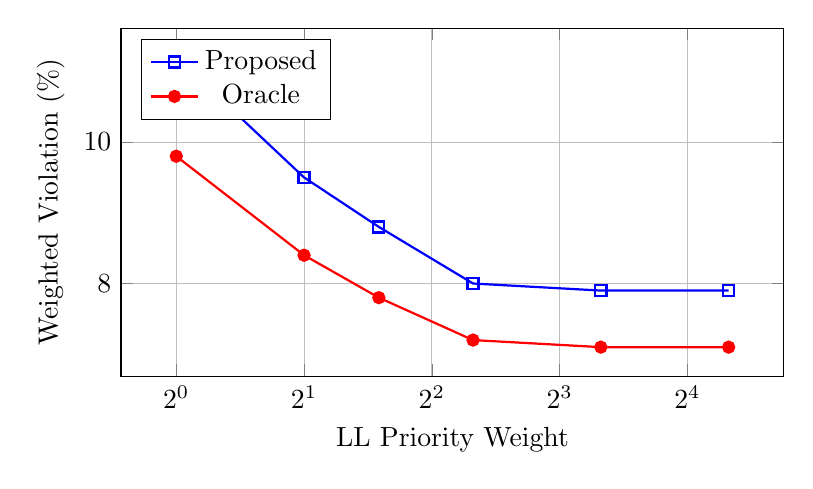
\begin{tikzpicture}
\begin{axis}[
    width=10cm, height=6cm,
    xlabel={LL Priority Weight},
    ylabel={Weighted Violation (\%)},
    grid=major,
    legend pos=north west,
    xmode=log,
    log basis x=2
]
\addplot[blue, mark=square, thick] coordinates {
    (1,11.2) (2,9.5) (3,8.8) (5,8.0) (10,7.9) (20,7.9)
};
\addplot[red, mark=*, thick] coordinates {
    (1,9.8) (2,8.4) (3,7.8) (5,7.2) (10,7.1) (20,7.1)
};
\legend{Proposed, Oracle}
\end{axis}
\end{tikzpicture}
\end{center}

\textbf{Finding:} Saturates at $w_{\text{LL}} \approx 5$ (KKT multiplier clips)
\end{frame}

\begin{frame}{Backup: Forecast Quality Metrics}
\begin{table}
\small
\begin{tabular}{lcccc}
\toprule
\textbf{Metric} & \textbf{Training} & \textbf{Validation} & \textbf{Test} & \textbf{3GPP Test} \\
\midrule
Pinball loss & 0.142 & 0.158 & 0.163 & 0.189 \\
Coverage@0.90 & 0.896 & 0.883 & 0.887 & 0.871 \\
Interval width (Mbps) & 187 & 203 & 211 & 245 \\
MAE (median) & 42.3 & 48.7 & 51.2 & 59.8 \\
\bottomrule
\end{tabular}
\end{table}

\textbf{Observations:}
\begin{itemize}
    \item Modest generalization gap (train $\rightarrow$ test)
    \item Coverage close to nominal (0.90)
    \item 3GPP: wider intervals, higher MAE (expected for transfer)
\end{itemize}
\end{frame}

\begin{frame}{Backup: Computational Complexity}
\begin{table}
\small
\begin{tabular}{lcc}
\toprule
\textbf{Component} & \textbf{Complexity} & \textbf{Time (Python)} \\
\midrule
Traffic generation & $\mathcal{O}(KT)$ & 0.8 ms/slot \\
Queue update & $\mathcal{O}(Q)$ & 0.2 ms/slot \\
Feature extraction & $\mathcal{O}(K \cdot F)$ & 0.1 ms \\
GBM forecast (8 cells) & $\mathcal{O}(K \cdot D \cdot L)$ & 0.8 ms \\
KKT solver & $\mathcal{O}(K \log K)$ & 0.4 ms \\
Service \& drops & $\mathcal{O}(Q)$ & 0.3 ms \\
\midrule
\textbf{Total per decision} & & \textbf{2.6 ms} \\
\bottomrule
\end{tabular}
\end{table}

$K$: cells, $T$: slots, $Q$: queue size, $F$: features, $D$: tree depth, $L$: leaves

\textbf{C++ estimate:} 10-20× faster $\rightarrow$ \textbf{0.1-0.3 ms} (acceptable)
\end{frame}

\begin{frame}[standout]
\begin{center}
\Huge Questions?
\end{center}
\end{frame}

\end{document}
